Знайдемо точне значення $Srn(C_4)$ для циклу на чотирьох вершинах, який зображений на рисунку \ref{c4:image}. Очевидно, що його ваги можна відновити за чотирма підспектрами, що є його ребрами.

\textbf{Приклад 3.} Для графа $C_4$, зображеного на рисунку \ref{ex3:image}, порахуємо його спектр.\\
\begin{figure}[H]
    \centering
    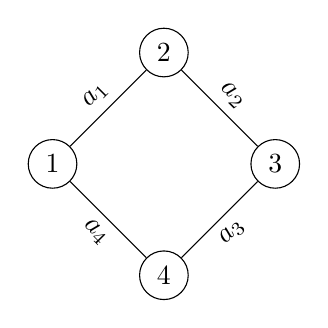
\begin{tikzpicture}[node distance={20mm}, main/.style = {draw, circle}]
    \node[main] (1) {$1$}; 
    \node[main] (2)[above right of=1] {$2$};
    \node[main] (3)[below right of=2] {$3$};
    \node[main] (4)[below left of=3] {$4$};
    \draw (1) -- node [midway, above, sloped] {$a_1$}(2);
    \draw (2) -- node [ above, midway, sloped] {$a_2$}(3);
    \draw (3) -- node [ below, midway, sloped] {$a_3$}(4);
    \draw (4) -- node [ below, midway, sloped] {$a_4$}(1);
    \end{tikzpicture}\\
    \caption{$C_4$}
    \label{ex3:image}
\end{figure}

Побудуємо матрицю суміжності $A$ для графа $C_4$ (рисунок \ref{ex3:image})

\begin{equation*}
A(G) =
\begin{pmatrix}
0 & a_1 & 0 & a_4\\
a_1 & 0 & a_2 & 0\\
0 & a_2 & 0 & a_3\\
a_4 & 0 & a_3 & 0
\end{pmatrix}
\end{equation*}

Знайдемо характеристичний многочлен за формулою (\ref{eq1})

\begin{multline*}
    P({\bf G})= 
\begin{vmatrix}
    \lambda & -a_1 & 0 & -a_4\\
    -a_1 & \lambda & -a_2 & 0\\
    0 & -a_2 & \lambda & -a_3\\
    -a_4 & 0 & -a_3 & \lambda
\end{vmatrix}
= \\
=\lambda
\begin{vmatrix}
    \lambda & -a_2 & 0\\
    -a_2 & \lambda & -a_3\\
    0 & -a_3 & \lambda
\end{vmatrix}
+ a_1
\begin{vmatrix}
    -a_1 & 0 & -a_4\\
    -a_2 & \lambda & -a_3\\
    0 & -a_3 & \lambda
\end{vmatrix}
+ a_4
\begin{vmatrix}
    -a_1 & 0 & -a_4\\
    \lambda & -a_2 & 0\\
    -a_2 & \lambda & -a_3
\end{vmatrix}
= \\
= \lambda^4-\lambda^2(a_1^2+a_2^2+a_3^2+a_4^2)+a_1^2a_3^2+a_2^2a_4^2-2a_1a_2a_3a_4 
\end{multline*}

\textit{Чи достатньо 3 підспектрів для відновлення усіх ваг $\bf C_4$?}
Запишемо характеристичний многочлен графа $\bf C_4$:
\begin{equation}\label{PC2}
    P_{\bf C_4}(\lambda) = \lambda^{4}-\lambda^{2}(a^2_{1} + a^2_{2} + a^2_{3} + a^2_{4})+(a^2_{1}a^2_{3} + a^2_{2}a^2_{4})-2a_{1}a_{2}a_{3}a_{4}
\end{equation}
Випишемо усі можливі варіанти з 3 підграфів:\\
1. $C_4$ і $2A_2$, що є сусідніми ребрами у графі.\\
2. $C_4$ і $2A_2$, що є паралельними ребрами у графі.\\
3. $C_4$ і $2A_3$, що перетинаються.\\
4. $C_4$ і $2A_3$, що не перетинаються.\\
5. $C_4$ і $A_3$, $A_2$, що перетинаються.\\
6. $C_4$ і $A_3$, $A_2$, що не перетинаються.\\
7. $3A_3$\\
8. $2A_3$, що перетинаються і $A_2$, що не входить у $2A_3$.\\
9. $2A_3$, що не перетинаються і $A_2$.\\
10. $A_3$ і $2A_2$.

Перевіримо кожен варіант.\\
1. Оберемо сусідні ребра (1;2)(2;3), зі спектра яких ми можемо відновити ваги $a_1, 
a_2$. Нехай $a_1 = b_1$, $a_2 = b_2$.
Тоді з характеристичного многочлена вихідного графа (\ref{PC2}) маємо значення таких коефіцієнтів: $a_3^2+a_4^2$, $b_1^2a_3^2+b_2^2a_4^2$, $a_3a_4$. Якщо $b_1^2=b_2^2$, то ми отримаємо симетричність. Тобто для графа ${\bf C_4}$(див. рисунок \ref{c4:image}) і для графа ${\bf C'_4}$(див. рисунок \ref{c42:image}), який дорівнює графу ${\bf C_4}$, але ваги ребер (1,4) і (3,4) поміняні місцями, тобто $w_{14} = a_3$ і $w_{34} = a_4$, значення $a_3^2+a_4^2$, $b_1^2a_3^2+b_2^2a_4^2$, $a_3a_4$ будуть однакові, але розташування ваг різне.
\input{graphs/С4_2}

2. Оберемо паралельні ребра (1;2)(3;4), зі спектра яких ми можемо відновити ваги $a_1, 
a_3$. Тоді з характеристичного многочлена вихідного графа маємо такі коефіцієнти: $a_2^2+a_4^2$, $a_2a_4$. Для довільного значення ваг $a_1,a_3$, маємо симетричність, тобто ситуацію, як у попередньому пункті.

3. Оберемо  такі $2A_3$, що перетинаються: $C_4-\{4\}$,$C_4-\{1\}$. 
Знайдемо їх характеристичні многочлени.
\begin{equation}\label{c4_4}
P_{{\bf C_4}-{4}}(\lambda) = \lambda^3 - \lambda(a_1^2+a_2^2)
\end{equation}
\begin{equation}
    P_{{\bf C_4}-{1}}(\lambda) = \lambda^3 - \lambda(a_2^2+a_3^2)
\end{equation}
Тоді з характеристичного многочлена вихідного графа(\ref{PC2}) і підграфів\\ $C_4-\{4\}$,$C_4-\{1\}$ маємо такі коефіцієнти: $a_1^2+a_2^2$,$a_2^2+a_3^2$,
$a_1^2+a_4^2$,$a_3^2+a_4^2$,$a_1^2a_3^2+a_2^2a_4^2$,$a_1a_2a_3a_4$, з яких не можна однозначно відновити усі ваги.

4. Оберемо  такі $2A_3$, що не перетинаються: $C_4-\{4\}$,$C_4-\{2\}$. 
Знайдемо характеристичний многочлен для ${\bf C_4}-\{2\}$:
\begin{equation}\label{c4_2}
    P_{{\bf C_4}-{2}}(\lambda) = \lambda^3 - \lambda(a_3^2+a_4^2)
\end{equation}
Тоді з характеристичного многочлена вихідного графа(\ref{PC2}) і підграфів:\\ ${\bf C_4}-\{4\}$(\ref{c4_4}),${\bf C_4}-\{2\}$(\ref{c4_2}) маємо такі коефіцієнти:$a_1^2+a_2^2$,$a_3^2+a_4^2$,
$a_1^2a_3^2+a_2^2a_4^2$,$a_1a_2a_3a_4$.

5. Оберемо $A_3$: $C_4-\{4\}$ і $A_2$: ребро(1;2). Зі спектра ребра відновлюємо вагу $a_1$, тоді зі  спектра ${\bf C_4}-\{4\}$(\ref{c4_4}), можна відновити вагу $a_2$.
Отримаємо таку саму ситуацію, як в першому пункті.

6. Оберемо $A_3$: $C_4-\{4\}$ і $A_2$: ребро(2;3). Зі спектра ребра відновлюємо вагу $a_4$, тоді зі  спектра $\bf C_4$(\ref{PC2}), коефіцієнту $a_1^2+a_2^2+a_3^2+a_4^2$, можна відновити вагу $a_4$, оскільки нам відомо значення $a_1^2+a_2^2$ зі спектра ${\bf C_4}-\{4\}$(\ref{c4_4}) і вага $a_3$. Отримаємо таку саму ситуацію, як в другому пункті.

7. Оберемо $A_3$: $C_4-\{4\}$, $C_4-\{1\}$, $C_4-\{2\}$. З їх характеристичних многочленів маємо такі коефіцієнти: $a_1^2+a_2^2$,$a_2^2+a_3^2$,$a_3^2+a_4^2$, яких недостатньо для відновлення ваг

8. Оберемо  такі $2A_3$: $C_4-\{4\}$,$C_4-\{1\}$ і $A_2$: ребро(1;4). Зі спектра ребра відновлюємо вагу $a_4$. Також маємо такі коефіцієнти з підспектрів:
$a_1^2+a_2^2$,$a_2^2+a_3^2$, яких недостатньо для відновлення ваг.

9. Оберемо  такі $2A_3$: $C_4-\{4\}$,$C_4-\{2\}$ і $A_2$: ребро$(1;2)$. Зі спектра ребра відновлюємо вагу $a_1$. Також відновлюємо $a_2$ зі спектра ${\bf C_4}-\{4\}$(\ref{c4_4}). Знаємо також коефіцієнт $a_3^2+a_4^2$, проте його недостатньо для відновлення ваг $a_3$ та $a_4$. 

10. Оберемо $A_3$: $C_4-\{4\}$ та ребра $(3;4),(4;1)$. З ребер відновлюємо ваги $a_3$,$a_4$ відповідно. Зі спектра ${\bf C_4}-\{4\}$(\ref{c4_4}) знаємо коефіцієнт $a_1^2+a_2^2$, проте його недостатньо для відновлення ваг $a_1$ та $a_2$.

